\chapter{Architektur}
\label{chap:Architektur}

\section{Module}
\label{sec:architektur.Module}

\begin{figure}[H]
\centering
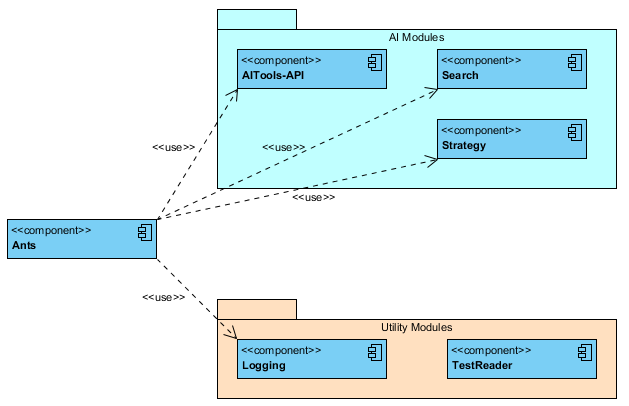
\includegraphics[width=0.9\textwidth]{91_bilder/modulesOverview}
\caption{Module}
\label{fig:modulesOverview}
\end{figure}

Abbildung \ref{fig:modulesOverview} zeigt die Gliederung des Bots in die verschiedenene Untermodule. Wir unterscheiden dabei zwischen den AI Modulen, welche die eigentliche AI-Logik enthalten, und den Utility Modulen, die Basisfunktionen wie Logging implementieren.

\paragraph{Ants:} Das Ants Modul enth�lt das Grundger�st des Bots und f�gt die anderen Module zu einem Ganzen zusammen. Es ist das einzige Modul, in dem Ants-spezifische Funktionalit�ten implementiert sind; die anderen sind generisch gehalten um die Wiederverwendbarkeit sicherzustellen. Das Ants Modul ist genauer dokumentiert im Kapitel \ref{sec:module.Ants}.

\paragraph{AITools-API:} Im API-Modul sind alle gemeinsamen Interfaces definiert, auf die die anderen Module zugreifen. Zum Teil ist hier auch Basis-Funktionalit�t implementiert, wie z.B. Distanzberechnungen auf einer Karte. Das API Modul ist genauer dokumentiert im Kapitel \ref{sec:module.API}.

\paragraph{Search:} Dieses Modul enth�lt unsere Implementationen zur Pfad- und Breitensuche. Ausf�hrliche Dokumentation dazu findet sich im Kapitel \ref{sec:module.Suchalgorithmen}.

\paragraph{Strategy:} Das Strategy-Module enth�lt strategische und taktische Algorithmen, insbesondere die Influence Map und das CombatPositioning. Ausf�hrliche Dokumentation dazu findet sich im Kapitel \ref{sec:module.StrategieTaktik}.

\paragraph{Logging:} Das Logging-Modul definiert ein flexibles Logging-Framework.Weitere Informationen dazu finden sich im Kapitel \ref{sec:module.Logging}.

\paragraph{TestReader:} Das TestReader-Modul besteht aus einer einzelnen Klasse, die aus den Log-Files der Ants-Spielengine Auswertungen lesen kann. Es ist genauer beschrieben im Kapitel \ref{sec:module.Testreader}.

\section{Modulabh�ngigkeiten}
\label{sec:architektur.Modulabh�ngigkeiten}


\begin{figure}[H]
\centering
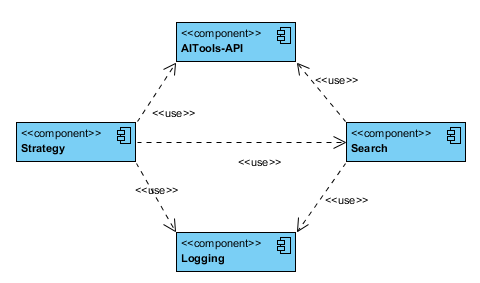
\includegraphics[width=0.8\textwidth]{91_bilder/modulesDependencies}
\caption{Modulabh�ngigkeiten}
\label{fig:modulesDependencies}
\end{figure}
Abbildung \ref{fig:modulesDependencies} zeigt die Abh�ngikeiten zwischen den Modulen. Die Module API und Logging sind unabh�ngig, w�hrend die beiden gr�sseren Module Abh�ngigkeiten auf API und Logging haben.
Die Abh�ngigkeit von Strategy auf Search r�hrt daher, dass die Influence Map mittels FloodFil Algorithmus aufgebaut wird, der im Search Modul implementiert ist.

\section{Externe Abh�ngigkeiten}
\label{sec:architektur.externeAbh�ngigkeiten}
Der Bot selber (also der Code, der von der Spielengine aufgerufen wird) hat keine externen Abh�ngigkeiten - dies w�re von den Regeln des Wettbewerbs auch gar nicht erlaubt gewesen. F�r ein paar andere Zwecke haben wir aber trotzdem auf externe Programmbibliotheken zur�ckgegriffen.

\begin{itemize}
\item
\textbf{JUnit \url{http://junit.org}:} F�r unsere zahlreichen Unit- und Funktions-Tests verwendeten wir Junit.
\item
\textbf{ClasspathSuite \url{http://johanneslink.net/projects/cpsuite.jsp}:} Da JUnit keine bequemen Weg bietet, alle Tests aus verschiedenen Projekten auf einmal auszuf�hren, verwendeten wir die ClasspathSuite, um die Tests direkt in Eclipse auszuf�hren.
\item
\textbf{Json-simple \url{http://code.google.com/p/json-simple/}:} Json-simple ist eine einfache Json-Parsing Bibliothek, die wir im TestReader verwenden, um die Json-Logs der Spielengine auszuwerten.
\end{itemize}